\documentclass[hidelinks]{article}

\title{Temperature And Winds In The Troposphere}
\author{Mihir Dasgupta, Indian Institute of Science, Bangalore (CAOS, IISc)}

\usepackage{hyperref}
\usepackage{tabto}
\usepackage{amsmath}
\usepackage{graphicx}
\usepackage{subcaption}
\usepackage{geometry}
\usepackage{titlesec}
\usepackage{xcolor}
\usepackage{cite}
\usepackage{mathtools}

\makeatletter
\setlength{\@fptop}{0pt}
\makeatother
\DeclareMathSizes{10.0}{12}{7}{7}

\geometry{a4paper, portrait, margin=0.5in}

\setcounter{secnumdepth}{4}

\hypersetup{%
  colorlinks=false,% hyperlinks will be black
  linkbordercolor=red,% hyperlink borders will be red
  pdfborderstyle={/S/U/W 1}% border style will be underline of width 1pt
}

\titleformat{\paragraph}
{\normalfont\normalsize\bfseries}{\theparagraph}{1em}{}
\titlespacing*{\paragraph}
{0pt}{3.25ex plus 1ex minus .2ex}{1.5ex plus .2ex}

\begin{document}
	\pagenumbering{roman}
	\maketitle
	\newpage	
	\tableofcontents

\newpage

\section{Introduction}
This report uses the data recorded by ESRL (Earth System Research Laboratory), under the \href{https://www.esrl.noaa.gov/psd/data/gridded/data.ncep.reanalysis.pressure.html}{Pressure NCEP/NCAR reanalysis} \cite{kalnay1996ncep}
\\\\
Some information about the datasets used in the charts below:
\begin{itemize}
	\item All of the data used for the calculations found in this report are monthly means of data recorded 4 times a day. 
	\item The data has been recorded for the last 71 years (since 1948)
	\item The two dimensional spatial data is recorded at a resolution of 2.5. This means, for example, that for every five latitudes, data is recorded twice.
\end{itemize}
\noindent The data is structured spatially across time, showing it to be four dimensional data. The data has been structured into a tree. For each data point in the structure, there are corresponding sub-points, usually a constant number at a specific level of the hierarchy. 
\\\\ Dimensions:
\begin{enumerate}
	\item Time- The data has been recorded since January 1948, 4 times a day. The data has been reduced to monthly means, each of which is a single item in the datasets used here.
	\\--- Unit: Months from January 1948
	\item Levels: This reanalysis uses pressure as a measure of altitude. (\ref{sec:measure}) The dataset considers altitude at 17 pressure levels, from 1000 mbar to 10 mbar. 
	\\--- Unit: Millibars
	\item Latitude: We use a resolution of 2.5, as previously explained. This gives us 72 latitudes recorded (180/2.5 = 72).
	\\--- Unit: Degrees Latitude
	\item Longitude: Similarly to latitude, we use a resolution of 2.5. This gives us 144 latitudes recorded (360/2.5 = 144).
	\\--- Unit: Degrees Longitude
\end{enumerate}
\textbf{Written under the direction of Dr. Jai Sukhatme, IISc}

\newpage
\section{Using Pressure As A Measure of Altitude}
\label{sec:measure}
\begin{figure}[h!]
	\centering
	\includegraphics[width=\linewidth]{../../altitudeVpressure/avp.png}
	\caption{Altitude to Pressure}
\end{figure}
\noindent
This sketch was made to create an idea of how altitude relates to air pressure, as pressure will often be used as a measure of altitude throughout this document. This sketch was made using the relationship of density of air as a function of altitude, as illustrated below:
\\\\
\begin{align*}
	f(h) &= p_0\left(1- \frac{Lh}{T_0}\right)^{\frac{gM}{RL}} \\
\end{align*}
where \\\\$p_{0}$ is the sea level standard atmospheric pressure, $1013.25$ $mbar,$ \\
$T_{0}$ is the sea level standard temperature, $288.15$ $K,$ \\
$g$ is the earth-surface gravitational acceleration, $9.80665$ $m/s^{2},$\\
$L$ is the temperature lapse rate, $0.0065$ $K/m,$\\
$R$ is the ideal (universal) gas constant, $8.31447$ $J/(K\cdot mol),$\\
$M$ is the molar mass of dry air, $0.0289644$ $kg/mol,$\\

\subsection{Hydrostatic equilibrium and its role in the atmosphere}
A fluid is said to be in hydrostatic balance or equilibrium when the flow velocity for each parcel of fluid is constant over time, or simply, is at rest. \cite{hydrostatic_equilibrium} In the atmosphere, this occurs when external forces, the most prominent being gravity, are in equilibrium with a pressure-gradient
 \newpage
\subsubsection{Pressure Gradient Force}
Consider a cuboidal parcel of fluid, with a height $dz$, a surface area $dA$ and a density $\rho$. While the atmosphere's shape is technically a hollowed-out sphere, the principle still holds. The cuboidal shape is being used for simplicity.

\begin{flalign}
Mass &= Density \cdot Volume && \\ 
&= \rho \cdot dz \cdot dA && 
%Force &= Mass \cdot Acceleration = Pressure \cdot Area && \\
%&= \rho \cdot dz \cdot \dA \cdot a = -dP \cdot dA &&
\end{flalign}

\begin{flalign}
Force &= Mass \cdot Acceleration = Pressure \cdot Area && \\
&= \rho \cdot dz \cdot dA \cdot a = -dP \cdot dA  && \\
&a = {\frac{-1}{\rho}} \cdot {\frac{dP}{dz}}
\end{flalign}

\begin{flalign}
Hydrostatic\ equation: {\frac{dP}{dz}} = {\frac{-\rho}{g}} &&
\end{flalign}
Substituting (6) in (5)
\begin{flalign}
a &= {\frac{-1}{\rho}} \cdot -\rho g&& \\
&= g
\end{flalign}
\\
\noindent The stated acceleration is the acceleration due to the pressure-gradient force. Force is exerted from high-pressure areas to low-pressure areas. In the atmosphere, this force would push upwards. Therefore, any mass of air in the atmosphere is in hydrostatic equilibrium, with the pressure-gradient force being driven by an acceleration equal to that caused by gravity.
\\\\
This property of the atmosphere has vital consequences. Had the pressure-gradient force been larger than gravity, the atmosphere would not be bound to the Earth and could diffuse into space. If it had been lower than gravity, the atmosphere would collapse into a thin, dense shell of air.

\newpage
\section{Module 1: Air Temperature In The Troposphere}
\subsection{Task 1: Air Temperature As A Function Of Latitude}
This exercise creates a general approximation of the air temperature across latitudes, and a rudimentary idea of how those temperatures change across altitudes.

\begin{figure}[h!]
	\centering
	\includegraphics[width=0.7\linewidth]{../../temperature/250v850/temp_plot_250v850.png}
	\caption{Temperature As A Function Of Latitude}
\end{figure}
\noindent In general, we see a peak in temperature near the 0$^\circ$ latitude, near the Equator, and a dip in temperature towards the poles, or near the 90$^\circ$ latitudes, both north and south.
\subsubsection{Changes In Temperature Latitudinally}
\begin{figure}[h!]
	\centering
	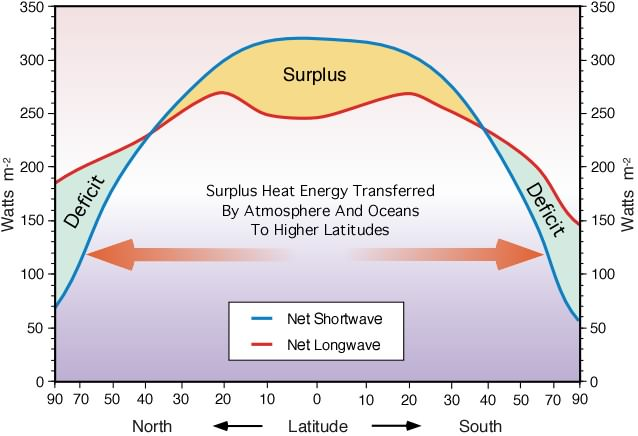
\includegraphics[width=0.8\linewidth]{olrVisr_lat.jpg}
	\caption{Outgoing Longwave Radiation and Incoming Solar Radiation Against Latitude}
\end{figure}
\noindent
The Earth's shape has a direct impact on the amount of solar energy each area on its surface receives. The Tropic Of Cancer receives the most sunlight, due to the the tilt of the Earth's axis. However, this does not imply it has the highest solar energy concentration on the Earth's surface. The rays of light it receives are indirect, and are therefore spread out over a large area. This means that the concentration of solar energy in a small area near this tropic would be lower than an area which received direct rays of light- the Equator.
\\\\
Additionally, there is a noteworthy latitudinal difference in the outgoing longwave radiation and the incoming solar radiation that helps to explain these findings. As shown in Figure 3 \cite{phdthesis}, there is a surplus of radiated energy from latitudes +30$^\circ$ to -30$^\circ$, and a deficit from those coordinates to their respective poles.
\\\\
As explained previously, different regions on the planet receive different energy concentrations per unit area. In the troposphere, there is a large amount of mixing of air, due to wind action and relatively denser air. In addition to ocean currents, this action carries away the surplus heat to the rest of the planet. Afterwards, the heat is radiated away from the planet in a manner somewhat proportional to the temperature at the area.
\\\\
That being said, there is a dip in longwave radiation near the equator. This is due to dense cloud cover near the area. Clouds are a type of aerosol, which reflect 63\% of the light they receive \cite{hatzianastassiou2007direct}, block outgoing radiation and therefore creates the aforementioned dip here.

\subsubsection{Changes In Temperature Across Altitudes}
Atmospheric pressure is the weight of air particles in the air exerting a downward force on the Earth's surface. Therefore, the atmospheric pressure is the greatest close to the Earth's surface. As with all fluid pressure, atmospheric pressure is high in a specific when there are more air particles in that area as compared to other sections of the body of air. Therefore, there are more air particles in lower regions of the troposphere. Consequently, there are less air particles as altitude increases.
\\\\
Incoming radiation passes through the atmosphere practically unabsorbed, and any heat in the troposphere is passed from the surface through conduction through air particles. As stated previously, the air is denser closer to the ground and becomes less so as altitude increases. Therefore, any conduction of heat reduces as direct contact and collisions of particles reduces, and the temperature decreases in the troposphere.  
\\\\
We see a similar waveform in the 250 millibar altitude as the 850 as the Sun's rays and the impact on areas stay roughly constant, therefore keeping latitudinal profiles relatively constant.

\subsection{Task 2: Seasonal Temperature Profiles As A Function Of Latitude}
This section explores changes in the above temperature with changes in seasons, each of which present different conditions whose consequences in temperature will be discussed here. The two seasons considered are the only universal ones, both of which show diametrically opposing conditions- winter and summer.
\subsubsection{850 Millibars}
\begin{figure}[h!]
	\centering
	\includegraphics[width=0.7\linewidth]{../../temperature/seasonal/ws850.png}
	\caption{Seasonal Temperature As A Function Of Latitude At 850 mbar}
\end{figure}
\noindent We see similar temperatures at regions closer to the Equator, but the temperature gap between seasons increases close to the South pole. Antarctica is a very large land mass surrounded by water. This means that the air above Antarctica changes temperature very quickly, owing to its solidity which generally conducts more heat. 
\\\\
Therefore, when there is only sunlight during the winters, the land mass stays heated and the air temperature rises. Similarly, the absence of sunlight, and consequently solar energy, the land mass stays cool and the air temperature dips.
\\\\
The Northern Hemisphere shows a constant difference in temperature between the seasons. This is because this hemisphere has more land than the southern hemisphere, compared to their respective volumes of water. Because there is more land, the temperature of the surface changes more often with fluctuations of solar energy at different times of day. 
\\\\
Generally, the winter is colder, and therefore, the air temperature is colder at this time as well. Similarly, the summer is warmer, and the air temperature is warmer at this time. This difference in air temperature is clearly manifested in the graph by the separation of the lines as compared to readings near the southern hemisphere.
\newpage
\subsubsection{250 Millibars}
\begin{figure}[h!]
	\centering
	\includegraphics[width=0.7\linewidth]{../../temperature/seasonal/ws250.png}
	\caption{Seasonal Temperature As A Function Of Latitude At 250 mbar}
\end{figure}
\noindent As expected, the shape of the graph does not change significantly at a higher altitude. However, the the temperature range increases dramatically from (20$^\circ$ to -40$^\circ$) to (40$^\circ$ to -80$^\circ$). This is because the air particles are fewer at the altitude and the solar energy does not dissipate to other particles, creating a balanced temperature. Therefore, at higher altitudes, the temperature rapidly heats and cools with a change in access to sunlight.
\subsection{Task 3: Temperature As A Function Of Latitude And Altitude}
The following figures provide us with a bird's-eye view of how air temperatures changed over altitudes across all latitudes. This was more of a general sketch that provides concrete basics in understanding temperature differences across the troposphere.
\subsubsection{Color Map}
\begin{figure}[h!]
	\centering
	\includegraphics[width=0.7\linewidth]{../../temperature/contour/color_map.png}
	\caption{Color Map}
\end{figure}
We observe phenomena previously seen and described in previous plots, all in one graph:
\begin{itemize}
	\item Temperature at any given level is at its extreme (other temperatures at this altitude considered) near the Equator.
	\item Temperature decreases as altitude increases.
	\item Temperature at any given is lowest at the South Pole.
\end{itemize}
\subsubsection{Contour Map}
\begin{figure}[h!]
	\centering
	\includegraphics[width=0.7\linewidth]{../../temperature/contour/contour_map.png}
	\caption{Contour Map}
\end{figure}
This plot was made to highlight the differences in temperature, where the average temperature drops below the freezing point of water, 0$^\circ$C. Near the poles, the average temperature is already below 0$^\circ$, but temperatures do not drop to this temperature before 600mbar, roughly 5000 ft or 1525 m. Refer to the graph in section 2 for these conversions(\ref{sec:measure}) 

\subsection{Task 4: Global Air Temperatures}
The following plots provided a much wider view of air temperature on the planet. Similarly to previous sections, we consider these temperatures at 2 distinct altitude levels- 250 mbar and 850 mbar. The images are generated across 4 projections:
\begin{enumerate}
	\item Equirectangular
	\item Orthographic
	\item South Polar Projection
	\item North Polar Projection
\end{enumerate}
\subsubsection{Equirectangular}	
\begin{figure}[h!]
	\centering
	\includegraphics[width=0.5\linewidth]{../../temperature/heatmap/Standard/850.png}
	\caption{Air Temperature at 850 mbar, Equirectangular Projection}
\end{figure}
\begin{figure}[h!]
	\centering
	\includegraphics[width=0.6\linewidth]{../../temperature/heatmap/Standard/250.png}
	\caption{Air Temperature at 250 mbar, Equirectangular Projection}
\end{figure}
\noindent The temperature bands become extremely clear with this projection- highlighting changes in temperature ranges across latitudes. The only anomaly found is the mass of cooler air over Eastern Europe at 250 millibars. This air is found to be cooler due to the large body of land found here. 
\newpage
\subsubsection{Orthographic}
This view is used to create visually-appealing maps without significant distortion. We made 360 perspectives with different central longitudes. 360 images were layered into a video at 12 frames per second, creating a 24 second video, for each level. For the sake of efficiency, a few significant frames have been attached below.
\paragraph{850 Millibars}
\begin{figure}[h!]
	\begin{subfigure}[b]{0.45545\linewidth}
		\centering
		\includegraphics[width=\linewidth]{../../temperature/heatmap/Orthographic/850/1.png}
		\caption{Orthographic Projection, Central Longitude: 0$^\circ$}
	\end{subfigure}
	\begin{subfigure}[b]{0.45545\linewidth}
		\centering
		\includegraphics[width=\linewidth]{../../temperature/heatmap/Orthographic/850/30.png}
		\caption{Orthographic Projection, Central Longitude: 30$^\circ$}
	\end{subfigure}
	\begin{subfigure}[b]{0.45545\linewidth}
		\centering
		\includegraphics[width=\linewidth]{../../temperature/heatmap/Orthographic/850/60.png}
		\caption{Orthographic Projection, Central Longitude: 60$^\circ$}
	\end{subfigure}
	\begin{subfigure}[b]{0.45545\linewidth}
		\centering
		\includegraphics[width=\linewidth]{../../temperature/heatmap/Orthographic/850/90.png}
		\caption{Orthographic Projection, Central Longitude: 90$^\circ$}
	\end{subfigure}
	\begin{subfigure}[b]{0.45545\linewidth}
		\centering
		\includegraphics[width=\linewidth]{../../temperature/heatmap/Orthographic/850/120.png}
		\caption{Orthographic Projection, Central Longitude: 120$^\circ$}
	\end{subfigure}
	\begin{subfigure}[b]{0.45545\linewidth}
		\centering
		\includegraphics[width=\linewidth]{../../temperature/heatmap/Orthographic/850/130.png}
		\caption{Orthographic Projection, Central Longitude: 130$^\circ$}
	\end{subfigure}
	\caption{Air Temperature at 850 Millibars, Orthographic Projection}
\end{figure}
\newpage
\paragraph{250 Millibars}
\begin{figure}[h!]
	\begin{subfigure}[b]{0.45545\linewidth}
		\centering
		\includegraphics[width=\linewidth]{../../temperature/heatmap/Orthographic/250/1.png}
		\caption{Orthographic Projection, Central Longitude: 0$^\circ$}
	\end{subfigure}
	\begin{subfigure}[b]{0.45545\linewidth}
		\centering
		\includegraphics[width=\linewidth]{../../temperature/heatmap/Orthographic/250/60.png}
		\caption{Orthographic Projection, Central Longitude: 60$^\circ$}
	\end{subfigure}
	\begin{subfigure}[b]{0.45545\linewidth}
		\centering
		\includegraphics[width=\linewidth]{../../temperature/heatmap/Orthographic/250/120.png}
		\caption{Orthographic Projection, Central Longitude: 120$^\circ$}
	\end{subfigure}
	\begin{subfigure}[b]{0.45545\linewidth}
		\centering
		\includegraphics[width=\linewidth]{../../temperature/heatmap/Orthographic/250/180.png}
		\caption{Orthographic Projection, Central Longitude: 180$^\circ$}
	\end{subfigure}
	\begin{subfigure}[b]{0.45545\linewidth}
		\centering
		\includegraphics[width=\linewidth]{../../temperature/heatmap/Orthographic/250/240.png}
		\caption{Orthographic Projection, Central Longitude: 240$^\circ$}
	\end{subfigure}
	\begin{subfigure}[b]{0.45545\linewidth}
		\centering
		\includegraphics[width=\linewidth]{../../temperature/heatmap/Orthographic/250/300.png}
		\caption{Orthographic Projection, Central Longitude: 300$^\circ$}
	\end{subfigure}
	\caption{Air Temperature At 250 Millibars, Orthographic Projection}
\end{figure}
\newpage
\subsubsection{South Polar Projection}
This projection provides us with an aerial view of the South Pole, highlighting unique atmospheric observations seen at the South Pole.
\begin{figure}[h!]
	\begin{subfigure}[b]{\linewidth}
		\centering
		\includegraphics[width=0.8\linewidth]{../../temperature/heatmap/SouthPolarStereo/850.png}
		\caption{Air Temperature At 850 Millibars, South Polar Projection}
	\end{subfigure}
	\begin{subfigure}[b]{\linewidth}
		\centering
		\includegraphics[width=0.8\linewidth]{../../temperature/heatmap/SouthPolarStereo/250.png}
		\caption{Air Temperature At 250 Millibars, South Polar Projection}
	\end{subfigure}
	\caption{Air Temperature Shown At A South Polar Projection}
\end{figure}
\subsubsection{North Polar Projection}
This projection provides us with a view of the North Poles, expounding on any special atmospheric conditions seen here, as compared to other parts of the globe.
\begin{figure}[h!]
	\begin{subfigure}[b]{\linewidth}
		\centering
		\includegraphics[width=0.8\linewidth]{../../temperature/heatmap/NorthPolarStereo/850.png}
		\caption{Air Temperature At 850 Millibars, North Polar Projection}
	\end{subfigure}
	\begin{subfigure}[b]{\linewidth}
		\centering
		\includegraphics[width=0.8\linewidth]{../../temperature/heatmap/NorthPolarStereo/250.png}
		\caption{Air Temperature At 250 Millibars, North Polar Projection}
	\end{subfigure}
	\caption{Air Temperature Shown At A North Polar Projection}
\end{figure}
\newpage
\section{Module 2: Zonal Winds In The Troposphere}
This module describes the charts related to zonal wind created during the span of the internship from June to July of 2019 using the monthly zonal wind recorded by ESRL.	
\subsection{Task 1: Zonal Wind As A Function Of Latitude}

This exercise was to create a general idea of the east-west wind, across the entire globe, considering two altitudes- 250 millibars, and 850 millibars. This also gives us an idea of how wind changes across different positions (latitudes) across the globe. The green line on the following chart is the wind profile at 250 millibars, at the red is the profile at 850 millibars.
\begin{figure}[h!] 
	\centering
	\includegraphics[width=0.7\linewidth]{../Zonal/general/plot_250v850.png}
	\caption{Zonal Wind As A Function Of Latitude}
\end{figure}

\noindent In general, we see larger waveforms on the 850 mbar altitude as lower pressures promote wind speeds.\\\\

\subsubsection{850 millibars} 
We see a sharp divot at the poles, which is a result of the polar easterlies. These speeds are lower as the temperature difference between the two air masses, one at the poles, and one at the 60$^\circ$ mark, is quite small. \\
We see a sharp increase in windspeed in the 30$^\circ$ to 60$^\circ$ and the -30$^\circ$ to -60$^\circ$ ranges as these are the ferrel cells. The reason these spikes are so large is that the temperature differences between the two air masses are so large. The warm air mass is rising directly above the equator, and the cold air mass is sinking near the 60$^\circ$ marks, which is sinking from the poles. \\\\
\noindent Moving closer to the equator, we see a small increase, which is air moving towards the west, as this is the warm air front moving to join the southern ferrel cell. Past the equator, we see a small divot which is the warm air front moving towards the northern ferrel cell.\\
We don't see a larger spike at the northern ferrel cell as the greater landmasses found can restrict the airflow near the surface due to increased surface friction. Instead, we see a plateau.

\subsubsection{250 millibars}
Similarly to the the same position on the 850 mbar level, we see a spike at the 60$^\circ$ degree mark. This spike is higher than the higher pressure level as wind speeds increase at lower pressure. \\\\
\noindent
We see no changes near the equator. This is because the winds formed near the equator in its 850 mbar counterpart are merging with the ferrel cells. This merging moves the winds away from the area. This means that the area is almost completely devoid of winds. \\

\subsection{Task 2: Seasonal Zonal Wind As A Function Of Latitude}
This exercise was to highlight the differences between latitudinal zonal wind across seasons and altitudes.
\subsubsection{Winter Vs Summer At 850 millibars}
\begin{figure}[h!]
	\centering
	\includegraphics[width=0.7\linewidth]{../Zonal/seasonal/ws850.png}
	\caption{Comparison at 850 millibars}
\end{figure}
Similarly to the 250 millibar level, we see a lower depression on the warm air mass at the southern ferrel cell. The winter has faster speeds at the northern ferrel cell due to a greater temperature difference. \\\\Unlike at the 250 mbar level, we don't see a notch in comparison at the 30$^\circ$ mark. This is because the wind during the winter still blows at the 850 mbar level. The wind blew up to a certain level, which evidently is somewhere between the 850 and 250 millibar levels. 

\subsubsection{Winter Vs Summer at 250 millibars}
\begin{figure}[h!]
	\centering
	\includegraphics[width=0.7\linewidth]{../Zonal/seasonal/ws250.png}
	\caption{Comparison at 250 millibars}
\end{figure}
\noindent We see incredibly high winds at the ferrel cells (-30$^\circ$ to -60$^\circ$, 30$^\circ$ to 60$^\circ$) here. This is due to the presence of ferrel cells, as earlier mentioned. \\
However, close to the southern ferrel cell, we see a higher plateau during the summer than the winter. This is because the warm front is stronger and therefore creates stronger winds. This also results in narrower and higher peaks for winter. \\
The greater divot during summer is due to the wind movement to the ferrel cells, which results in a smaller peak at the northern ferrel cell.

\newpage
\subsection{Task 3: Zonal Wind As A Function Of Latitude and Altitude}
The following figures gave us an idea of how the wind changed over altitudes across all latitudes. This was more of a general sketch that allowed us to zoom out and look at the whole picture.
\\\\There are 2 main controlled variables that we averaged out for the sake of a cleaner plot- time and longitude.
The independent variables were the latitude and level- which meant for every latitude there was a corresponding level which carried a single value.
\subsubsection{Color Map}
\begin{figure}[h!]
	\centering
	\includegraphics[width=0.7\linewidth]{../Zonal/contour/color_map.png}
	\caption{Color Map}
\end{figure}
\noindent We find that the winds are at their highest speeds around the positive and negative 50$^\circ$ marks. This is because this is at the centre of the ferrel cells, which has the highest speeds amongst all the weather cells. Looking at that line, we do see a higher wind speed at any level at this latitude. The reason we see increasing and therefore decreasing wind speeds, with the 50$^\circ$ marks at the centre is because of the presence of the ferrel cells.\\We see an eastward wind near the equator which is the circulation that provides the warm air front to each of the two ferrel cells. We do see a stronger eastward wind at the -20$^\circ$ mark. This is because the wind moves faster here which results in a higher average wind at the southern ferrel cell as compared to its northern counterpart.
\subsubsection{Contour Map}
\begin{figure}[h!]
	\centering
	\includegraphics[width=0.7\linewidth]{../Zonal/contour/contour_plot.png}
	\caption{Contour Map}
\end{figure}
\noindent This plot highlighted the differences between the westward and eastward winds. This gave us a clearer picture of the boundaries between the various wind systems. \\A noteworthy observation is that only the southern polar cell is distinguishable. This is due to the temperature differences between the two polar cells because of the Earth's tilted axis.
\newpage
\subsection{Task 4: Global Zonal Winds}
The following plots gave us a much wider view of zonal winds on the planet. Similarly to previous sections, we consider profiles at two altitudes- 850 and 250 millibars. The images are generated across two projections- the equirectangular projection and the north polar projection.
\subsubsection{Equirectangular Projection}
\begin{figure}[h!]
	\begin{subfigure}[b]{\linewidth}
		\centering
		\includegraphics[width=0.8\linewidth]{../Zonal/heatmap/Standard/standard_850.png}
		\caption{Equirectangular Projection, 850 millibars}
	\end{subfigure}
	\begin{subfigure}[b]{\linewidth}
		\centering
		\includegraphics[width=0.8\linewidth]{../Zonal/heatmap/Standard/standard_250.png}
		\caption{Equirectangular Projection, 250 millibars}
	\end{subfigure}
	\caption{Equirectangular Projection}
\end{figure}
\newpage
\noindent At low levels, across the globe, we see more inconsistent wind speeds- regardless of its direction- There are very few long stretches wherein any wind remains constant. This is due to the influence of friction caused by varying features exhibited on the Earth's crust. 
More specifically, one of the major influences of friction is whether the surface is land or water. As the land is harder, rougher and introduces more variation in terms of altitude, the average friction exerted over land would be higher than that exerted over water.
\\\\
Starting from the equator, we see two eastward moving winds, both slightly above and below the equator- the northeast and southeast trade winds, respectively. This is because of the low pressure system created by its intense heating. The warm air, heated at the equator, flows outwards towards the poles. \\\\However, there is a build up of air at the horse latitudes, due to the curvature of the Earth's surface, creating a high pressure region in these areas. The high pressure results in the air sinking, which separates, flowing north and south. Because of the rotation of the earth and the coriolis force, air moves towards the west in the northern hemisphere, while moving northwards. The opposite holds true for air moving towards the south in the northern hemisphere. 
\\\\
This means that the air above the northern horse latitude and the air beneath the southern horse latitude move towards the west- the westerlies. As for the air surrounding the equator, they move towards the east- creating the trade winds.
\\\\
The westerlies and the sinking air from the poles collide near the 60$^\circ$ marks. They push each other upwards, creating an area of low pressure near the surface at these latitudes. As they move towards the right in the northern hemisphere, it creates a wind moving towards the west- called the polar easterlies.
\\\\
Moving on, there are instances where we see a stronger wind than their counterparts, whether they be towards the east or west, or as the other hemisphere's counterpart:\\\\
1. \underline{Eastern Trade Wind, 250 millibars:} Circulations often multiply when the wind at its lower altitude is not as fast, which also applies conversely. The eastern trade wind over the 850 millibars is not as strong due to the broken up presence of land which meant that the varying altitude shows massive variation in friction. 
\\\\
2. \underline{Western Trade Wind, 850 millibars:} There are concentrations of higher wind speeds over the Atlantic and Pacific Ocean, due to the reduction of friction seen over seas. 
\\\\
3.  \underline{Southern Westerlies:} The southern westerlies have higher wind speeds across both altitudes due to the presence of the Southern Ocean which is almost completely uninterrupted by land, the only one being South America.
\newpage
\subsubsection{North Polar Projection}
\begin{figure}[h!]
	\begin{subfigure}[b]{\linewidth}
		\centering
		\includegraphics [width=0.8\linewidth]{../Zonal/heatmap/North_Polar_Stereo/north850.png}
		\caption{North Polar Stereographic Projection, 850 millibars}
	\end{subfigure}
	\begin{subfigure}[b]{\linewidth}
		\centering
		\includegraphics[width=0.8\linewidth]{../Zonal/heatmap/North_Polar_Stereo/north250.png}
		\caption{North Polar Stereographic Projection, 250 millibars}
	\end{subfigure}
	\caption{North Polar Stereographic Projection}
\end{figure}
\noindent We see stronger polar easterlies near the surface, that also expand to latitudes closer to the equator. This is because the wind moves further to the south as altitude increases, in addition to the fact that the westerlies expand northwards as we increase altitudes.
\newpage
\subsubsection{Orthographic}
This view is used to create visually-appealing maps without significant distortion. We made 360 perspectives with different central longitudes. Links to the full videos can be found below. 360 images were layered into a video at 12 frames per second, creating a 24 second video, for each level.
\paragraph{850 Millibars}
\begin{figure}[h!]
	\centering
	\begin{subfigure}[b]{0.45545\linewidth}
		\includegraphics[width=\linewidth]{../Zonal/heatmap/850mbar/0.png}
		\caption{Orthographic Projection, Central Longitude: 0$^\circ$}
	\end{subfigure}
	\begin{subfigure}[b]{0.45545\linewidth}
		\includegraphics[width=\linewidth]{../Zonal/heatmap/850mbar/60.png}
		\caption{Orthographic Projection, Central Longitude: 60$^\circ$}
	\end{subfigure}
	\begin{subfigure}[b]{0.45545\linewidth}
		\includegraphics[width=\linewidth]{../Zonal/heatmap/850mbar/120.png}
		\caption{Orthographic Projection, Central Longitude: 120$^\circ$}
	\end{subfigure}
	\begin{subfigure}[b]{0.45545\linewidth}
		\includegraphics[width=\linewidth]{../Zonal/heatmap/850mbar/180.png}
		\caption{Orthographic Projection, Central Longitude: 180$^\circ$}
	\end{subfigure}
	\begin{subfigure}[b]{0.45545\linewidth}
		\includegraphics[width=\linewidth]{../Zonal/heatmap/850mbar/240.png}
		\caption{Orthographic Projection, Central Longitude: 240$^\circ$}
	\end{subfigure}
	\begin{subfigure}[b]{0.45545\linewidth}
		\includegraphics[width=\linewidth]{../Zonal/heatmap/850mbar/300.png}
		\caption{Orthographic Projection, Central Longitude: 300$^\circ$}
	\end{subfigure}
	\caption{Orthographic Projection At 850 Millibars}
\end{figure}
\newpage
\paragraph{250 Millibars}
\begin{figure}[h!]
	\centering
	\begin{subfigure}[b]{0.45545\linewidth}
		\includegraphics[width=\linewidth]{../Zonal/heatmap/250mbar/0.png}
		\caption{Orthographic Projection, Central Longitude: 0$^\circ$}
	\end{subfigure}
	\begin{subfigure}[b]{0.45545\linewidth}
		\includegraphics[width=\linewidth]{../Zonal/heatmap/250mbar/60.png}
		\caption{Orthographic Projection, Central Longitude: 60$^\circ$}
	\end{subfigure}
	\begin{subfigure}[b]{0.45545\linewidth}
		\includegraphics[width=\linewidth]{../Zonal/heatmap/250mbar/120.png}
		\caption{Orthographic Projection, Central Longitude: 120$^\circ$}
	\end{subfigure}
	\begin{subfigure}[b]{0.45545\linewidth}
		\includegraphics[width=\linewidth]{../Zonal/heatmap/250mbar/180.png}
		\caption{Orthographic Projection, Central Longitude: 180$^\circ$}
	\end{subfigure}
	\begin{subfigure}[b]{0.45545\linewidth}
		\includegraphics[width=\linewidth]{../Zonal/heatmap/250mbar/240.png}
		\caption{Orthographic Projection, Central Longitude: 240$^\circ$}
	\end{subfigure}
	\begin{subfigure}[b]{0.45545\linewidth}
		\includegraphics[width=\linewidth]{../Zonal/heatmap/250mbar/300.png}
		\caption{Orthographic Projection, Central Longitude: 300$^\circ$}
	\end{subfigure}
	\caption{Orthographic Projection At 250 Millibars}
\end{figure}
\newpage
\section{Module 3: Meridional Winds In The Troposphere}
This module describes the charts related to north-south (meridional) wind created during the span of the internship from June to July 2019 using the mean monthly meridional wind recorded by ESRL.

\subsection{Task 1: Meridional Wind As A Function Of Latitude}
This exercise was to create a general idea of how the north-south wind changes across the globe. We measured the wind across two altitudes, one near the surface (850 millibars) and one at lower pressures (250 millibars).\\\\
We do see a pattern across the 250 and 850 millibar winds- the crest of any smaller wave coincides with the trough of the other wind's waves.  In general, this shows us that there are currents that are created with altitude that are not majorly influenced by other factors.
\begin{figure}[h!]
	\centering
	\includegraphics[width=0.7\linewidth]{../Meridional/latitudinal_profile/htVlat.png}
	\caption{Meridional Wind As A Function of Latitude}
\end{figure}
\subsubsection{850 Millibars}
In general, we see uneven waveforms across all latitudes. This is due to the increased influence of friction and temperature differences across bodies of water and land. With changes in the ratios between land and water bodies, we see changes in meridional wind, which causes the general wave forms seen across both of the altitudes.
A noteworthy observation is the immense spikes in meridional wind near the Antarctic. There are numerous warm currents in the Southern Ocean, which, when combined with the colder currents produced near the Antarctic, created extremely strong northwards winds. This also results in the increase of zonal westerly speeds in the South.
\subsubsection{250 Millibars}
We see cleaner waveforms at this level due to lower friction and temperature differences. We see a deep depression near the Pacific, called the Walker Cell. This is caused due to the temperature difference between the Western and the Eastern Pacific Ocean. The Western side is heated by warmer ocean countries coming from the warm waters of the China Sea.

\subsection{Task 2: Seasonal Meridional Wind As A Function Of Latitude}
Seasonal plots show cleaner plots as seasonal changes in wind direction are prominent.
\subsubsection{850 Millibars}
\begin{figure}[h!]
	\centering
	\includegraphics[width=0.8\linewidth]{../Meridional/seasonal/ws850.png}
	\caption{Seasonal Meridional Wind, 850 Millibars}
\end{figure}
\noindent The variations occur in intervals- where the summer has a strong northward wind, winter has a strong southward wind. This is due to the changes in temperature differences caused by seasonal changes in ocean currents. When they collide with temperatures over land, The wind changes in direction. 
\subsubsection{250 Millibars}
\begin{figure}[h!]
	\centering
	\includegraphics[width=0.8\linewidth]{../Meridional/seasonal/ws250.png}
	\caption{Seasonal Meridional, 250 Millibars}
\end{figure}
\noindent We observe similar results at this higher altitude, which points us to the idea that meridional wind does not change significantly with altitude.
\newpage
\subsection{Task 3: Meridional Wind As A Function of Latitude And Altitude}
\subsubsection{Colour Map}
\begin{figure}[h!]
	\centering
	\includegraphics[width=0.7\linewidth]{../Meridional/contour/colormap.png}
	\caption{Colour Map}
\end{figure}
\noindent In general, this shows us that northward and southward wind appears in regions, changing in key latitudes such as the tropics. We see strong winds near the surface (925 Millibars) as the temperature difference are stronger here. However, a reasonable inference is that these winds are not as strong at the surface (1000 Millibars) as the meridional winds are offset by friction at the surface.
\subsubsection{Contour Map}
\begin{figure}[h!]
	\centering
	\includegraphics[width=0.7\linewidth]{../Meridional/contour/contour_plot.png}
	\caption{Contour Map}
\end{figure}
\noindent This plot highlights the differences between the strong northward and southward winds, which highlights the strong southward winds are near the surface, and. much higher, at the 150-250 Millibar levels.
\subsection{Task 4: Global Meridional Winds}
These following plots are categorized into various projections. The data is plotted spatially on two dimensions at various levels.
The plots are made at various projections to highlight different zones.
\subsubsection{Equirectangular Projection}
\begin{figure}[h!]
	\begin{subfigure}[b]{\linewidth}
		\centering
		\includegraphics[width=0.8\linewidth]{../Meridional/heatmap/Standard/850.png}
		\caption{Equirectangular Projection, 850 Millibars}
	\end{subfigure}
	\begin{subfigure}[b]{\linewidth}
		\centering
		\includegraphics[width=0.8\linewidth]{../Meridional/heatmap/Standard/250.png}
		\caption{Equirectangular Projection,  250 Millibars}
	\end{subfigure}
	\caption{Equirectangular Projection}
\end{figure}
\noindent Across both of the levels, we see northward and southward wind in a checked pattern. This is due to the temperature differences between land and bodies of water. They do not flow directly north to south due to the Coriolis force.
\subsubsection{North Polar Stereographic Projection}
\begin{figure}[h!]
	\begin{subfigure}[b]{\linewidth}
		\centering
		\includegraphics[width=0.85\linewidth]{../Meridional/heatmap/North_Polar_Stereo/850.png}
		\caption{North Polar Stereographic Projection, 850 Millibars}
	\end{subfigure}
	\begin{subfigure}[b]{\linewidth}
		\centering
		\includegraphics[width=0.85\linewidth]{../Meridional/heatmap/North_Polar_Stereo/250.png}
		\caption{North Polar Stereographic Projection, 250 Millibars}
	\end{subfigure}
	\caption{North Polar Stereographic Projection}
\end{figure}
\noindent At the 850 millibar level, we see alternating northward and southward wind. Whereas, at the 250 millibar level, we see curving wind speeds. This is due to the multiplication of the effect of the Coriolis force.
\subsubsection{South Polar Stereographic Projection}
\begin{figure}[h!]
	\begin{subfigure}[b]{\linewidth}
		\centering
		\includegraphics[width=0.85\linewidth]{../Meridional/heatmap/South_Polar_Stereo/850.png}
		\caption{South Polar Stereographic Projection, 850 Millibars}
	\end{subfigure}
	\begin{subfigure}[b]{\linewidth}
		\centering
		\includegraphics[width=0.85\linewidth]{../Meridional/heatmap/South_Polar_Stereo/250.png}
		\caption{South Polar Stereographic Projection, 250 Millibars}
	\end{subfigure}
	\caption{South Polar Stereographic Projection}
\end{figure}
\noindent We see similar results at the South Pole as we did at the North Pole- while they travel in alternating directions at lower altitudes. They curve at higher altitudes.
\newpage
\subsubsection{Orthographic}
This view is used to create visually-appealing maps without significant distortion. We made 360 perspectives with different central longitudes. Links to the full videos can be found below. 360 images were layered into a video at 12 frames per second, creating a 24 second video, for each level.
\paragraph{850 Millibars}
\begin{figure}[h!]
	\centering
	\begin{subfigure}[b]{0.45545\linewidth}
		\includegraphics[width=\linewidth]{../Meridional/heatmap/850mbar/0.png}
		\caption{Orthographic Projection, Central Longitude: 0$^\circ$}
	\end{subfigure}
	\begin{subfigure}[b]{0.45545\linewidth}
		\includegraphics[width=\linewidth]{../Meridional/heatmap/850mbar/60.png}
		\caption{Orthographic Projection, Central Longitude: 60$^\circ$}
	\end{subfigure}
	\begin{subfigure}[b]{0.45545\linewidth}
		\includegraphics[width=\linewidth]{../Meridional/heatmap/850mbar/120.png}
		\caption{Orthographic Projection, Central Longitude: 120$^\circ$}
	\end{subfigure}
	\begin{subfigure}[b]{0.45545\linewidth}
		\includegraphics[width=\linewidth]{../Meridional/heatmap/850mbar/180.png}
		\caption{Orthographic Projection, Central Longitude: 180$^\circ$}
	\end{subfigure}
	\begin{subfigure}[b]{0.45545\linewidth}
		\includegraphics[width=\linewidth]{../Meridional/heatmap/850mbar/240.png}
		\caption{Orthographic Projection, Central Longitude: 240$^\circ$}
	\end{subfigure}
	\begin{subfigure}[b]{0.45545\linewidth}
		\includegraphics[width=\linewidth]{../Meridional/heatmap/850mbar/300.png}
		\caption{Orthographic Projection, Central Longitude: 300$^\circ$}
	\end{subfigure}
	\caption{Orthographic Projection At 850 Millibars}
\end{figure}
\newpage
\paragraph{250 Millibars}
\begin{figure}[h!]
	\centering
	\begin{subfigure}[b]{0.45545\linewidth}
		\includegraphics[width=\linewidth]{../Meridional/heatmap/250mbar/0.png}
		\caption{Orthographic Projection, Central Longitude: 0$^\circ$}
	\end{subfigure}
	\begin{subfigure}[b]{0.45545\linewidth}
		\includegraphics[width=\linewidth]{../Meridional/heatmap/250mbar/60.png}
		\caption{Orthographic Projection, Central Longitude: 60$^\circ$}
	\end{subfigure}
	\begin{subfigure}[b]{0.45545\linewidth}
		\includegraphics[width=\linewidth]{../Meridional/heatmap/250mbar/120.png}
		\caption{Orthographic Projection, Central Longitude: 120$^\circ$}
	\end{subfigure}
	\begin{subfigure}[b]{0.45545\linewidth}
		\includegraphics[width=\linewidth]{../Meridional/heatmap/250mbar/180.png}
		\caption{Orthographic Projection, Central Longitude: 180$^\circ$}
	\end{subfigure}
	\begin{subfigure}[b]{0.45545\linewidth}
		\includegraphics[width=\linewidth]{../Meridional/heatmap/250mbar/240.png}
		\caption{Orthographic Projection, Central Longitude: 240$^\circ$}
	\end{subfigure}
	\begin{subfigure}[b]{0.45545\linewidth}
		\includegraphics[width=\linewidth]{../Meridional/heatmap/250mbar/300.png}
		\caption{Orthographic Projection, Central Longitude: 300$^\circ$}
	\end{subfigure}
	\caption{Orthographic Projection At 250 Millibars}
\end{figure}
\newpage
\section{Anomalies: Zonal And Meridional Wind}
This section highlights the differences between average winds and winds for certain months at specified altitudes. There is a colour map on each of the following plots of the section- which is the average magnitude across the globe .We express these winds in terms of vectors, with the following components:
\begin{itemize}
	\item x-component: Zonal Wind (East-West Wind)
	\item y-component: Meridional Wind (North-South Wind)
\end{itemize} 
For every month, we will look at two altitudes- 250 millibars and 850 millibars.
\subsection{January Vs Average Wind}
January is used for standard anomalies for all of the winter months.
\subsubsection{850 Millibars}
\begin{figure}[h!]
	\centering
	\includegraphics[width=0.85\linewidth]{../Anomalies/250anomalies/jan850.png}
	\caption{January Wind Vs Average Wind, 850 Millibars}
\end{figure}
\newpage
\noindent The major difference is the northward wind with a slight westward deviation, at the 60$^\circ$ N latitude. This is due to the lower temperature during the winter. The Equator, while cooler, still receives a significant amount of sunlight, while the poles receive almost none.\\
This creates a larger than average temperature difference between the North Pole and the Equator. This difference forces the wind northwards at a higher-than-average speed.
\subsubsection{250 Millibars}
\begin{figure}[h!]
	\centering
	\includegraphics[width=0.85\linewidth]{../Anomalies/250anomalies/jan250.png}
	\caption{January Wind Vs Average Wind, 250 Millibars}
\end{figure}
\noindent We see similar changes in direction at this level, as meridional wind, unlike zonal wind, does not change with altitude. The wind veers eastwards at this level, as the zonal winds are extremely strong here.
\newpage
\subsection{July Vs Average Wind}
July is used for standard anomalies for all of the summer months.
\subsubsection{850 Millibars}
\begin{figure}[h!]
	\centering
	\includegraphics[width=0.95\linewidth]{../Anomalies/250anomalies/july850.png}
	\caption{July Wind Vs Average Wind, 850 Millibars}
\end{figure}
\noindent We see a convergence of wind at the 30$^\circ$S latitude. Air moves southwards from the equator, and northwards from the Southern Ocean. The high heat at the equator during the summer causes the air to rise and spread out into lower pressure areas, such as the tropics, in this case. The Southern Ocean has a higher than average temperature, causing the rising air to move towards the lower pressure tropics.  
\\\\
The Equator's sheer heat causes the air above it to move quickly up to the tropics, to a lower pressure area.
\subsubsection{250 Millibars}
\begin{figure}[h!]
	\centering
	\includegraphics[width=0.95\linewidth]{../Anomalies/250anomalies/july250.png}
	\caption{July Wind Vs Average Wind, 250 Millibars}
\end{figure}
\noindent We see similar winds at this altitude, with the exception of the wind veering eastwards. The reason behind this is that the change is meridional, and meridional wind does not change with altitude. The wind veers eastward because at this height, zonal wind influences the wind, forcing it eastward.
\newpage

\bibliography{documentation}{}
\bibliographystyle{plain}

\end{document}